This thesis explains in detail the process undertaken to collect references for the systematic review of literature (SRL), highlighting the search queries, the outcomes of those queries, and the relative data sources. 

\section{Research Methodology}
\label{sec:resmetodologies}
The research methodology adopted in this thesis is the \emph{comprehensive systematic literature review} a research methodology because it offers a structured and meticulous process for identifying, assessing, and examining existing resources to explore a specific research topic or question. The procedure is meticulously described in \citeauthor{budgen_performing_2006} (2006). In addition, the snowballing approach proposed by \citeauthor{wohlin_guidelines_2014} (2014) was used to integrate papers resulting from search queries.
\begin{figure}
\begin{center}
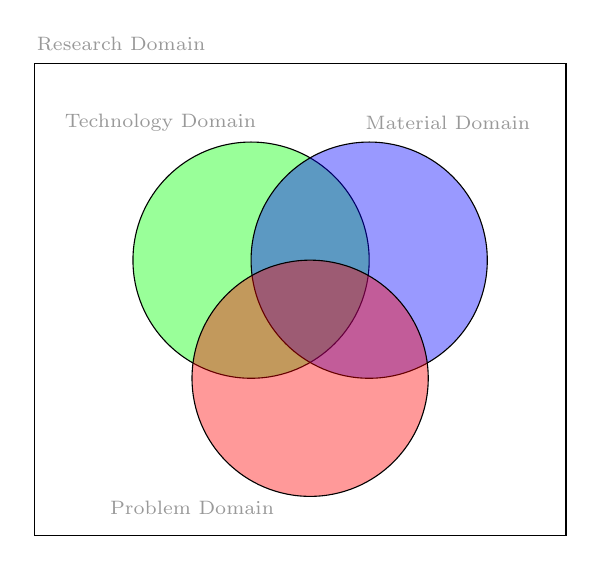
\begin{tikzpicture}[scale=0.5]
	\begin{scope} [fill opacity = .4]
    \draw (-7,6) rectangle (6.5,-6);
    \draw[fill=green, draw = black] (-1.5,1) circle (3);
    \draw[fill=blue, draw = black] (1.5,1) circle (3);
    \draw[fill=red, draw = black] (0,-2) circle (3);
    \node at (-4.8,6.5) {\scriptsize{Research Domain}};
    \node at (-3.8,4.5) {\scriptsize{Technology Domain}};
    \node at (3.5,4.5) {\scriptsize{Material Domain}};
    \node at (-3,-5.3) {\scriptsize{Problem Domain}};
    \end{scope}
\end{tikzpicture}
\end{center}
\caption{Research domain.} \label{fig:resdomains}
\end{figure}

\paragraph{Research terms.}
To identify the relevant keywords and terms for the research, I defined the research domain, identifying the most commonly used words and their synonyms. Then, using the snowballing approach \cite{wohlin_guidelines_2014}, I found other related terms, leveraging the references from papers discovered with the initial queries. The schema of the abovementioned method is described in Fig. \ref{fig:snowballing}. Three domains were identified: the technological domain, outlined by the PBF processes discussed throughout the thesis; the materials domain associated with the PBF processes; and the problem domain, focusing on detecting hot spots using ML-based methods. Search queries were structured using terms in the intersection of these three domains (Fig. \ref{fig:resdomains}). Below are the terms found during this first phase
\begin{itemize}
    \item \textbf{Technological domain:} powder bed fusion, L-PBF, PBF, electron beam melting, selective laser sintering, SLS, EBM, EB-PBF.
    \item \textbf{Material domain:} metal, alloy, metal powder.
    \item \textbf{Problem domain:} hot spot, detection, machine learning, ML.
\end{itemize}

\paragraph{Research sources} In an SLR, selecting appropriate resources to search for material is vital. All available literature relevant to the scope of the thesis was searched using the following online data banks:
\begin{itemize}
    \item Google Scholar (\href{https://scholar.google.com}{https://scholar.google.com})
    \item IEEE Xplore digital library (\href{https://ieeexplore.ieee.org}{https://ieeexplore.ieee.org})
    \item Scopus (\href{https://www.scopus.com/}{https://www.scopus.com/})
\end{itemize}

\paragraph{Performed queries.} This paragraph reports all the queries used on the different sources for the research. \\[1.5ex]
Query performed on Scopus:
\begin{tcolorbox}
\footnotesize
((Powder AND bed AND fusion) OR PBF OR L-PBF OR (electron AND beam AND melting) OR (selective AND laser AND sintering) OR SLS OR EBM OR EB-PBF) AND (metal OR alloy OR (metal AND powder)) AND  (hot AND spot*) AND (ML OR (machine AND learning)) AND ((defect* OR anomal*) AND detection) AND ((additive AND manufacturing) OR AM)
\end{tcolorbox}
Since IEEE Xplore digital does not have the structured query Scopus does, multiple queries were performed.
\begin{tcolorbox}
\footnotesize
"All Metadata":"powder bed fusion" AND "metal" AND "hot spot*" AND "detection"
\end{tcolorbox}
\begin{tcolorbox}
\footnotesize
"All Metadata":"electron beam melting" AND "metal" AND "hot spot*" AND "detection"
\end{tcolorbox}
\begin{tcolorbox}
\footnotesize
"All Metadata":"selective laser sintering" AND "metal" AND "hot spot*" AND "detection"
\end{tcolorbox}
The same queries were also used on Google Scholar.

\section{Research Result and Selection Process.}
\label{sec:resresults}
\begin{figure}
    \centering
    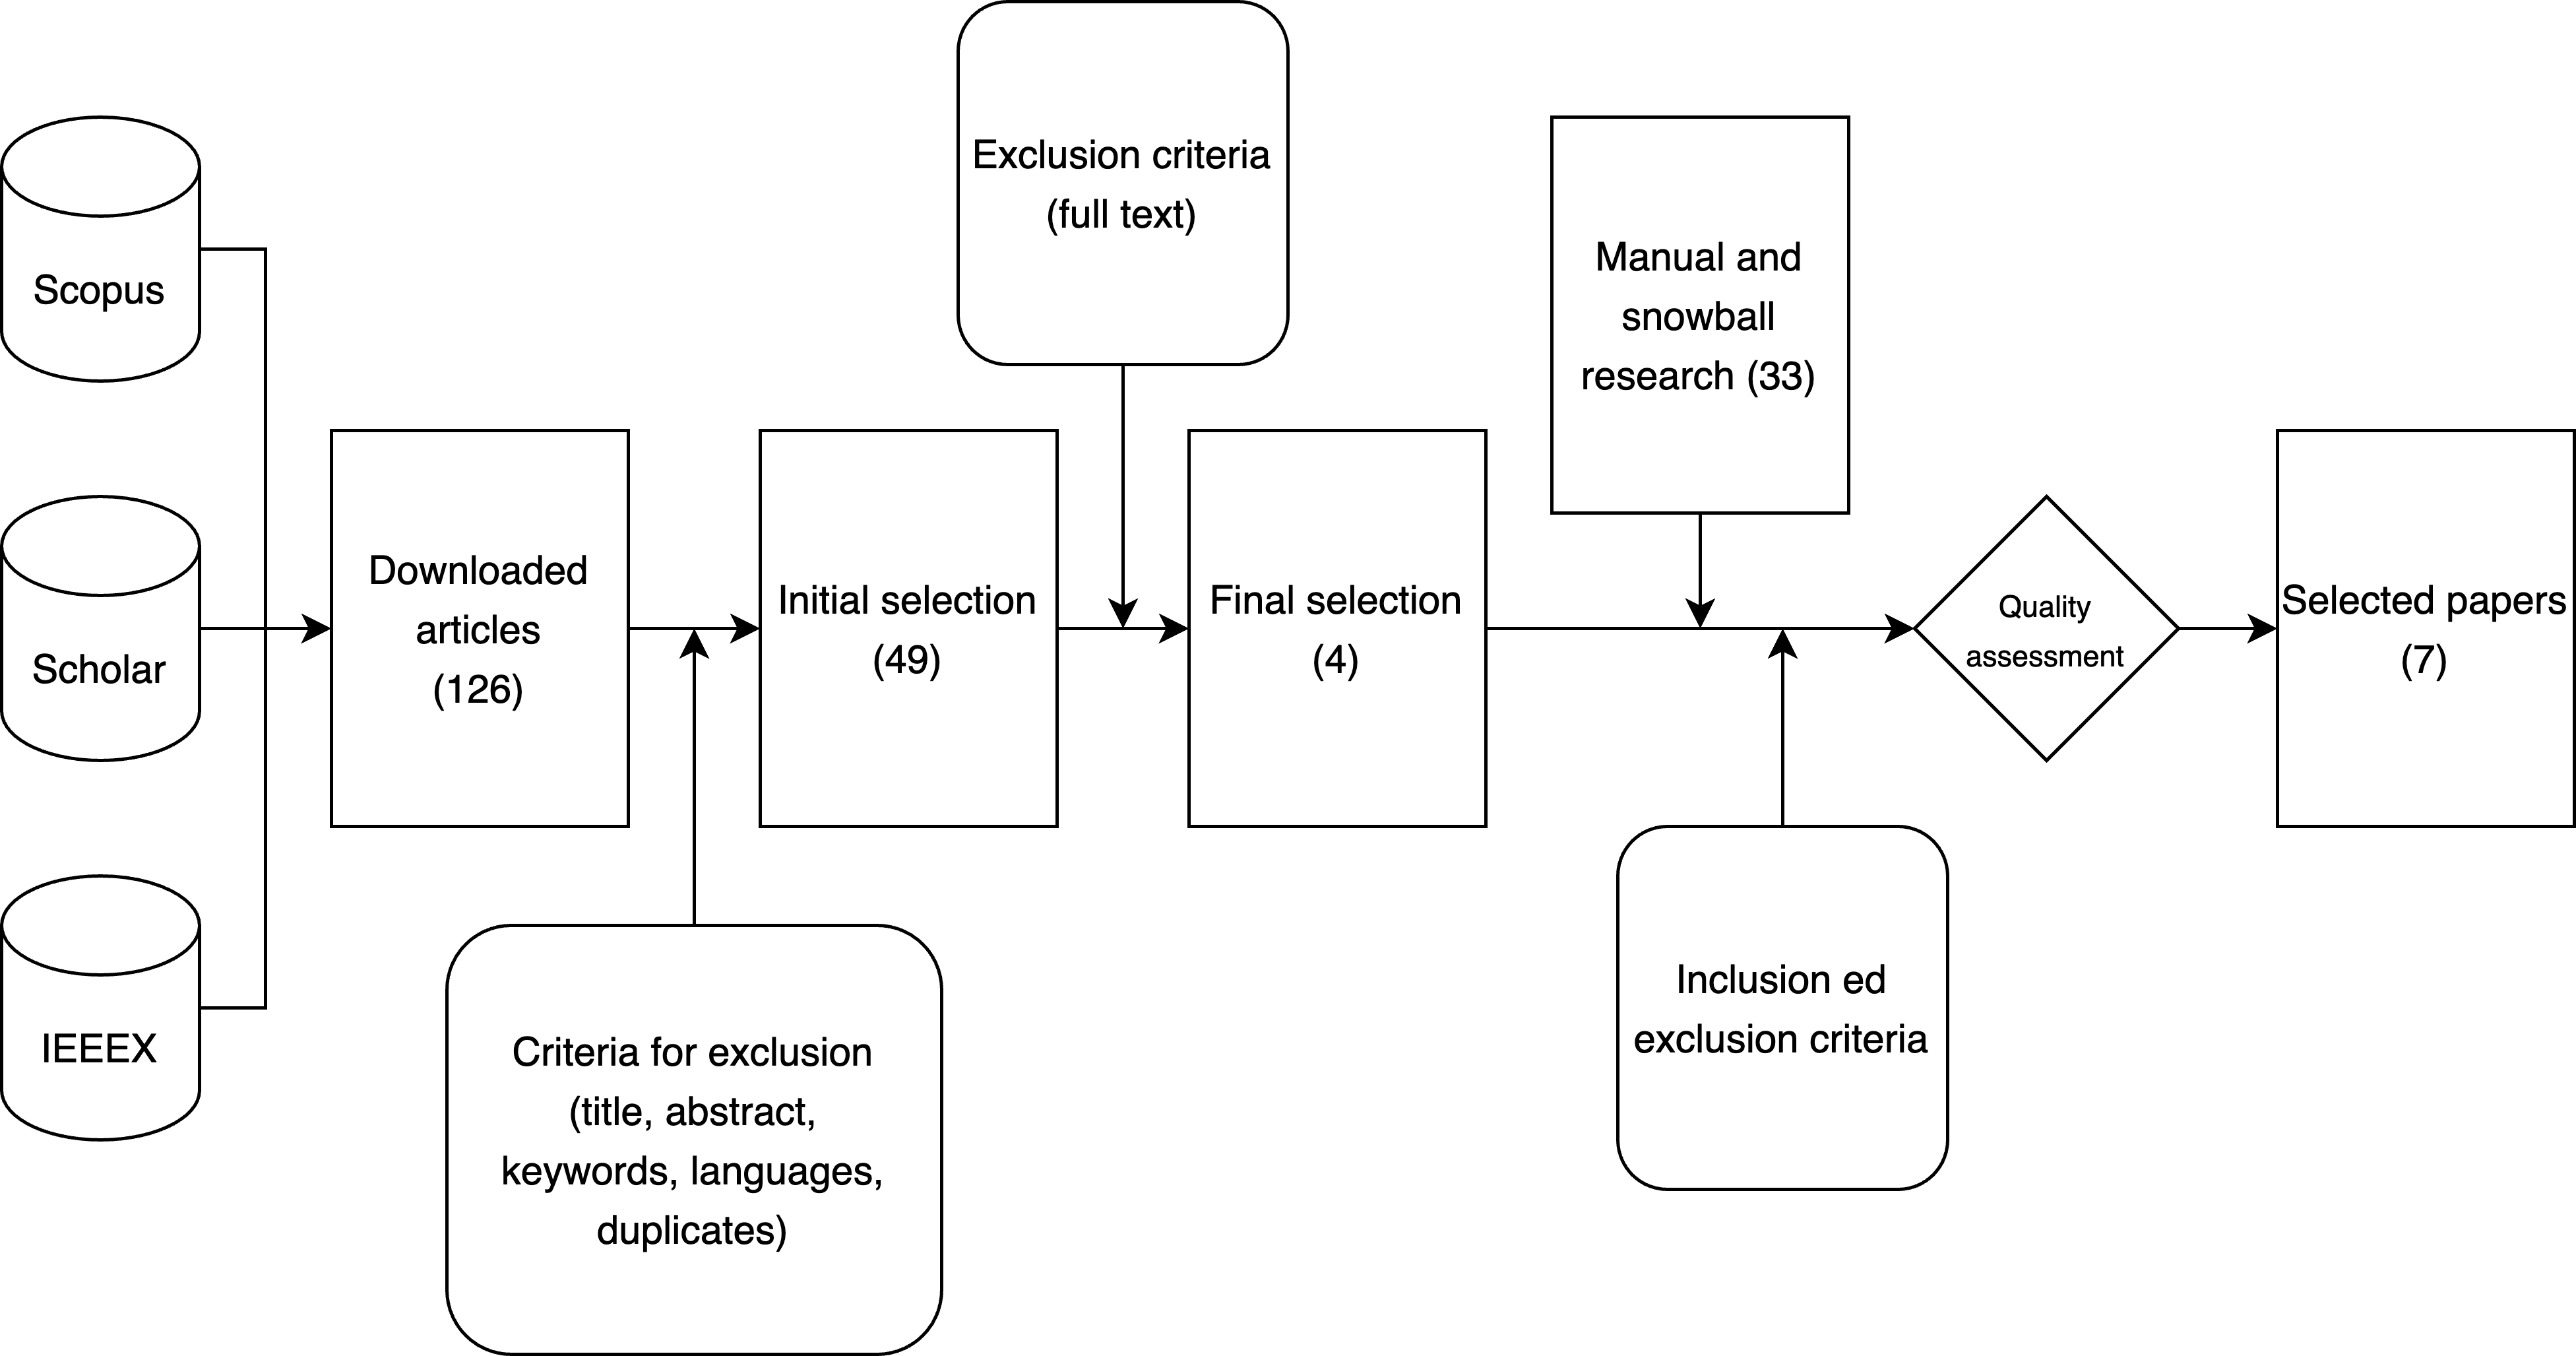
\includegraphics[scale=0.1]{Images/selection.png}
    \caption[Papers selection procedure.] {Papers selection procedure.}
    \label{fig:selection}
\end{figure}
During the SLR, exclusion, and inclusion criteria were used to select the final papers for the research. An article has to meet the following criteria to be useful in answering our research questions.
\paragraph{Inclusion criteria.} Below are the inclusion criteria used during the SLR:
\begin{itemize}
    \item All the articles, written in English, report machine learning or deep learning techniques for  hot spot detection;
    \item All papers, journals, conferences, workshops, and short papers but books.
    \item All articles about the systematic review of possible defects in PBF.
\end{itemize}
\paragraph{Exclusion criteria.} On the other hand, the following exclusion criteria were also used in the SLR:
\begin{itemize}
    \item Papers about defect detection methods other than machine learning or deep learning;
    \item Papers that are not available in their whole;
    \item Papers written in a language besides English;
    \item Papers in a state besides "Final Release".
\end{itemize}

For the last point, these papers are used to write \emph{Chapter ~\ref{ch:defects}} and perform the snowballing procedure explained before.

\begin{figure}
    \centering
    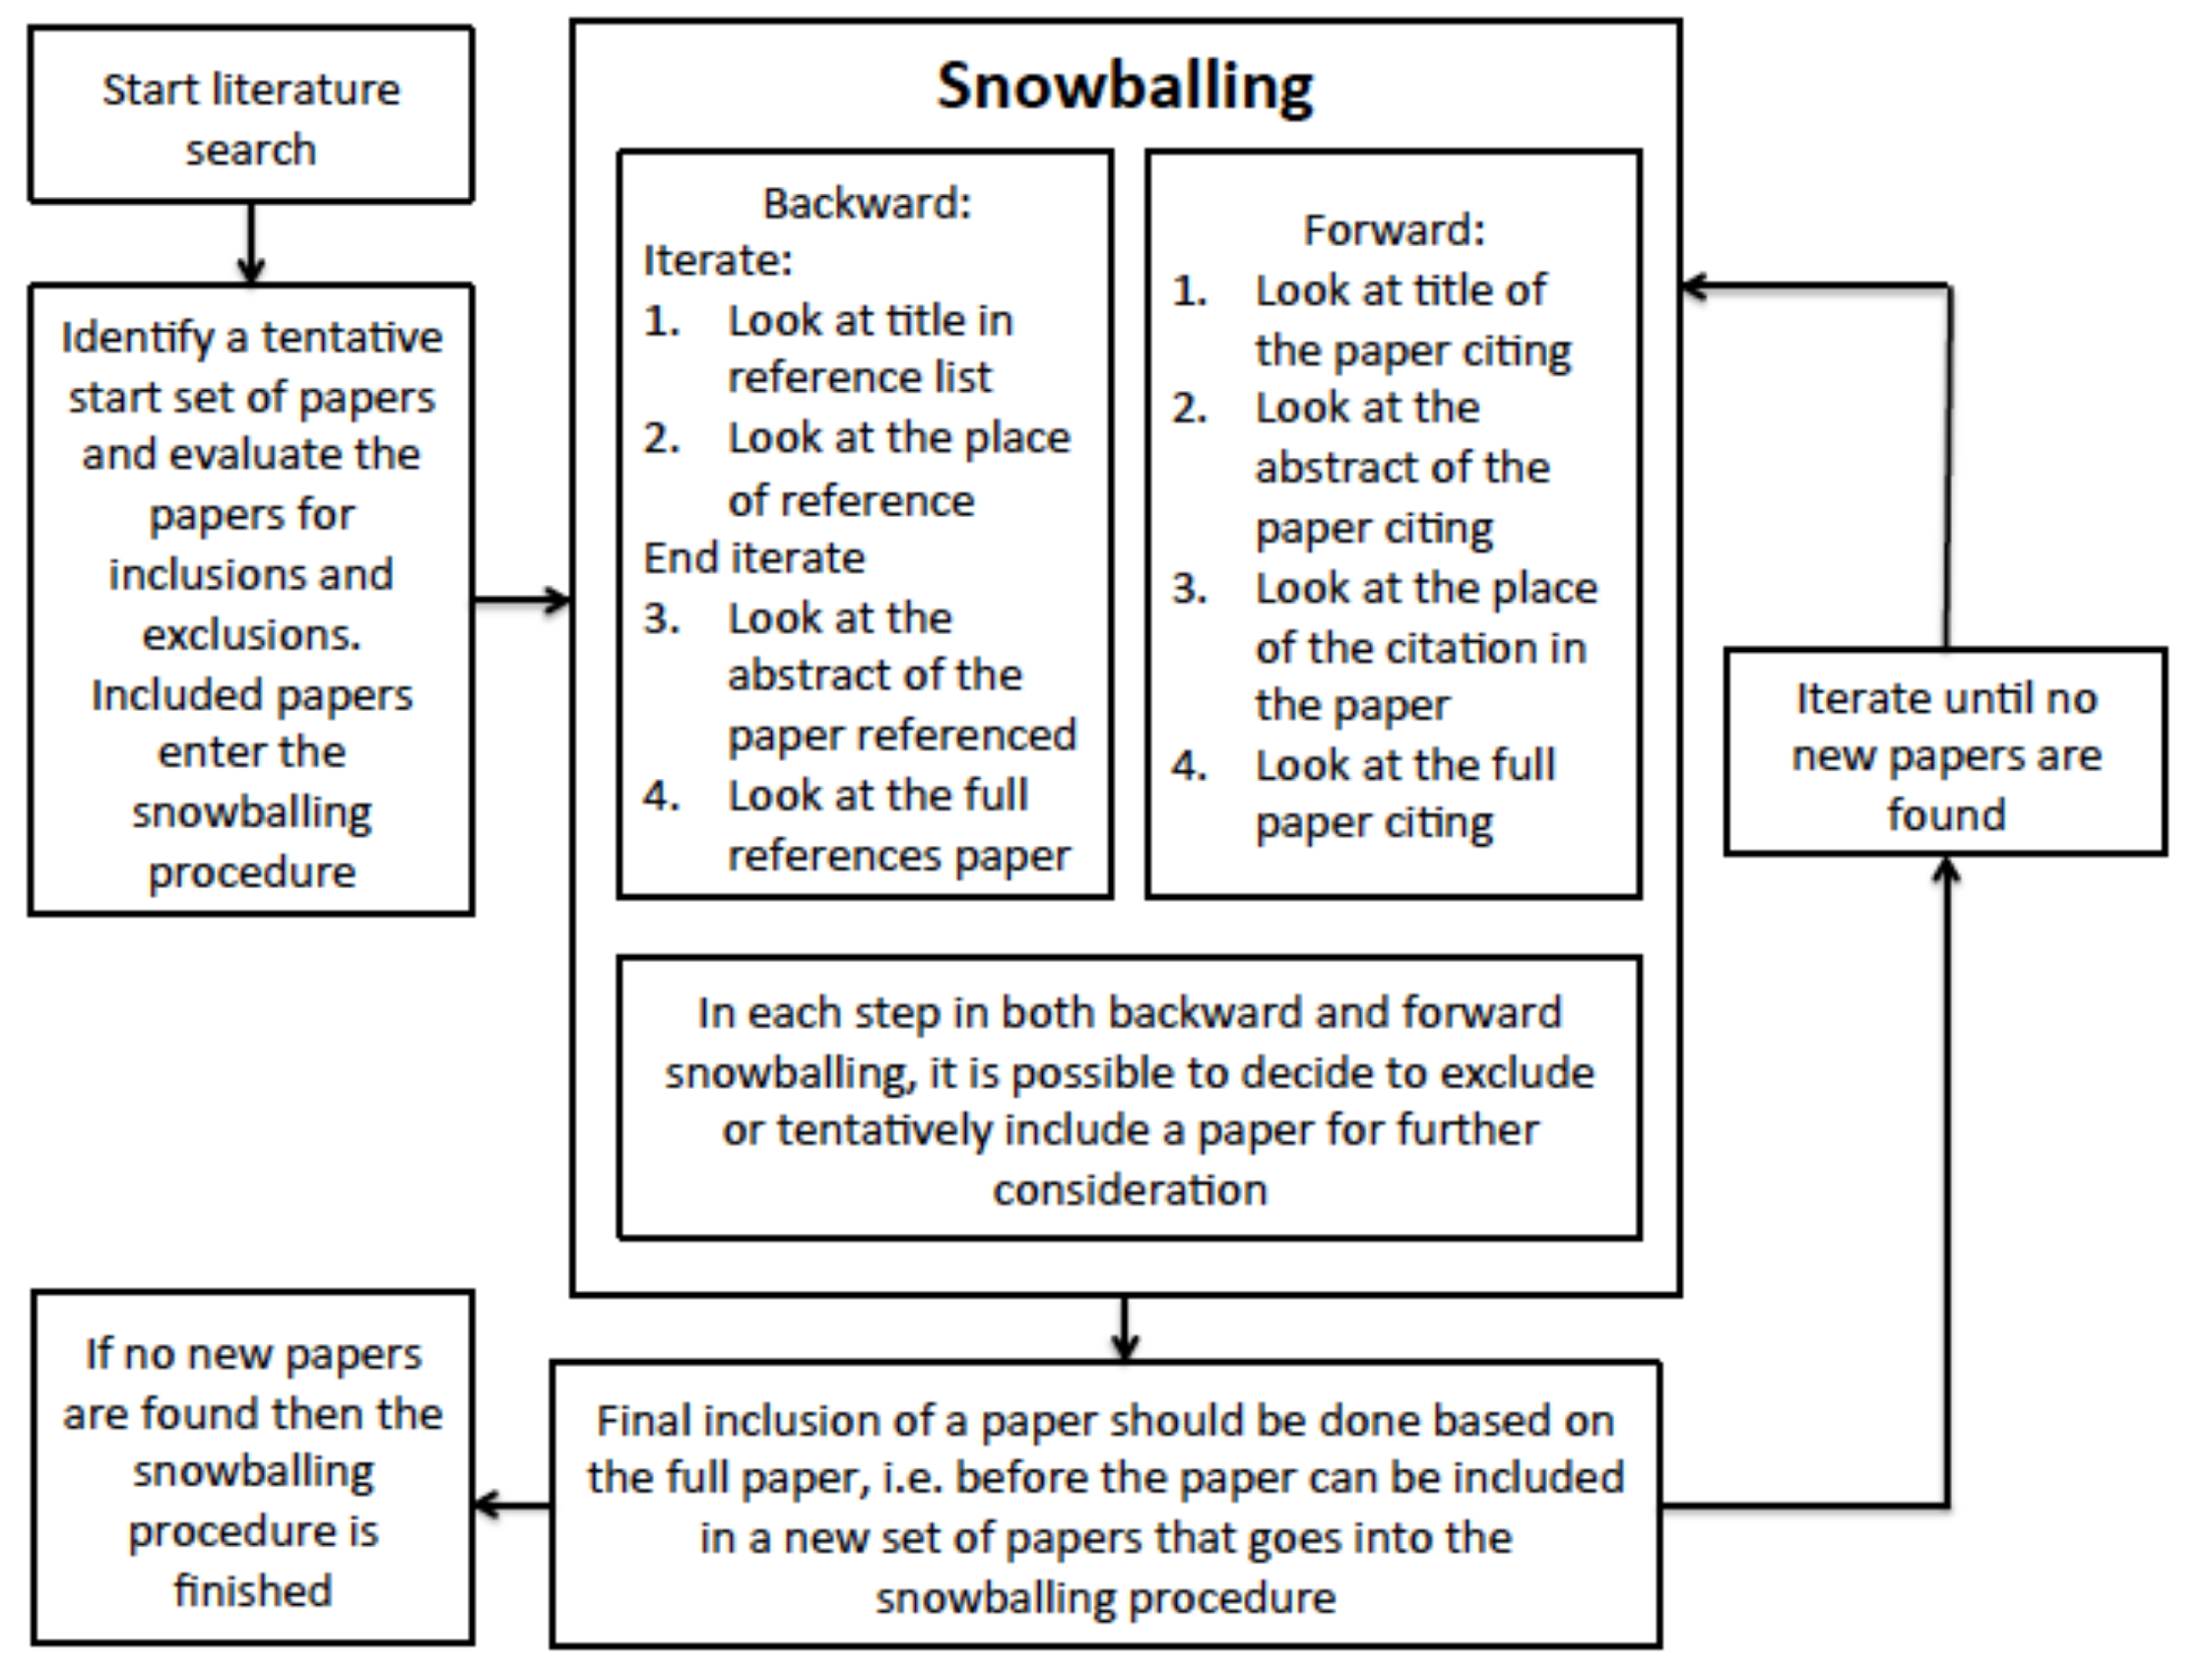
\includegraphics[scale=0.25]{Images/snowballing.png}
    \caption[Snowballing procedure.] {The schema of the snowballing procedure \cite{wohlin_guidelines_2014}.}
    \label{fig:snowballing}
\end{figure}